\documentclass[10pt,twocolumn,letterpaper]{article}

\usepackage{cvpr}
\usepackage{times}
\usepackage{epsfig}
\usepackage{graphicx}
\usepackage{color}
\usepackage{transparent}
\usepackage{caption}
\usepackage{subcaption}
\usepackage{amsmath}
\usepackage{amssymb}
\usepackage{mathtools}
\newcommand{\norm}[1]{\left\lVert #1 \right\rVert}
\DeclarePairedDelimiter\abs{\lvert}{\rvert}

% Include other packages here, before hyperref.

% If you comment hyperref and then uncomment it, you should delete
% egpaper.aux before re-running latex.  (Or just hit 'q' on the first latex
% run, let it finish, and you should be clear).
%\usepackage[pagebackref=true,breaklinks=true,letterpaper=true,colorlinks,bookmarks=false]{hyperref}

\cvprfinalcopy % *** Uncomment this line for the final submission

\def\cvprPaperID{} % *** Enter the 3DV Paper ID here
\def\httilde{\mbox{\tt\raisebox{-.5ex}{\symbol{126}}}}

% Pages are numbered in submission mode, and unnumbered in camera-ready
%\ifcvprfinal\pagestyle{empty}\fi
\setcounter{page}{1}
\begin{document}

%%%%%%%%% TITLE
\title{Structure from Motion with RGB-D}

\author{Seonwook Park \\
ETH Zurich \\
{\tt\small spark@student.ethz.ch}
% For a paper whose authors are all at the same institution,
% omit the following lines up until the closing ``}''.
% Additional authors and addresses can be added with ``\and'',
% just like the second author.
% To save space, use either the email address or home page, not both
\and
Yifan Wang \\
ETH Zurich \\
{\tt\small yifan.wang@student.ethz.ch}
}

\maketitle
%\thispagestyle{empty}

%%%%%%%%% ABSTRACT
\begin{abstract}
   A structure from motion pipeline is constructed using C++, OpenCV, Ceres
   solver, and PCL. This includes the acquisition of data, extraction and
   matching of features, estimation of pairwise camera pose using depth data,
   transformation of estimates into a global coordinate frame, and performing
   bundle adjustment on all data. This pipeline incorporates depth data taken
   from a Microsoft Kinect in pairwise camera pose estimation to improve the
   final 3D reconstruction, which simplifies the conventional pipeline and improves the robustness of the result. Furthermore the inclusion of depth data in the bundle adjustment was attempted and compared with the result using a standard cost function.
\end{abstract}

%%%%%%%%% BODY TEXT
\section{Introduction}

Structure from Motion (SfM) concerns the recreation of a real environment
through the inferring of motion from images \cite{varga2008practical}. (1)
First, a 3D object or environment is imaged from multiple different
perspectives. (2) In each image, it is possible to find keypoints via feature
detection algorithms such as SIFT and SURF, and calculate descriptors with which
correspondences can be found in other images. (3) After finding corresponding
pairs, the relative pose of each camera can be inferred in various ways.

With early implementations of SfM, keypoints are projected into 3D space and
optimisation algorithms such as RANSAC and Levenberg-Marquardt are used to find
the homography or perspective transformation between two image planes. With the
advent of low-cost commercial depth sensing cameras, it is now possible to
incorporate depth information in hopes to improve or speed this procedure up. An
example is the Microsoft Kinect, which casts and reads an infra-red pattern
which is used to calculate depth values per pixel imaged \cite{zhang2012microsoft}.

For problems of corresponding 2D points (image plane) and 3D points (using depth
values), one can use PnP or Perspective-n-Point algorithms \cite{d2013p3p}. A P3P
algorithm uses a minimum of 3 data points to infer the relative pose between a
pair of cameras. There are optimised PnP algorithms available, which when
coupled with RANSAC can discard outliers and estimate relative camera pose
accurately \cite{lepetit2009epnp}.

Once an initial estimate for relative camera pose is made, this can be optimised
via bundle adjustment, an optimisation step operated on sparse keypoints from
the perspective of all cameras. To do so, (4) pairwise camera pose estimates
need to be transformed into a single coordinate system. This is achieved through
the construction of a minimum spanning tree with cameras as nodes and the
existence of corresponding pairs as edges. When camera pose estimates are
relative to a single coordinate system, it is possible to project keypoints into
the coordinate system from the perspective of each camera. Minimising this
reprojection is the (5) bundle adjustment step.

A final model can be constructed by projecting all known data into 3D space
using final camera pose estimates. In such a way a dense 3D reconstruction is
possible. The alignment of RGB-D data in the final reconstruction is
representative of the SfM pipeline's performance.

This study concerns the use of depth data in hopes to improve the accuracy of
the final 3D reconstruction output. This is done both in the pairwise camera
pose estimation step as well as the bundle adjustment step where depth data
is introduced into the minimisation problems.


%-------------------------------------------------------------------------

\section{Methodology}

\begin{figure*}[ht]
\begin{center}
   \includegraphics[width=0.9\linewidth]{figures/pipeline.pdf}
\end{center}
\caption{Overview of Structure from Motion pipeline}
\label{fig:pipeline}
\end{figure*}

As outlined in the previous sections, our structure from motion pipeline is
composed of 5 main steps as shown in figure \ref{fig:pipeline}.

\begin{enumerate}
\item Data acquisition
\item Feature detection and matching
\item Pairwise camera pose estimation
\item Transform to global coordinate system
\item Bundle adjustment
\end{enumerate}

It is important to note that the acquired images in this case is RGB-D and is
acquired using a Microsoft Kinect (first generation).

The pipeline is implemented in C++. Third party libraries used include OpenCV
3.0, Ceres Solver and PCL 1.8.

%-------------------------------------------------------------------------

\subsection{Data acquisition}
\begin{figure*}
\begin{center}
   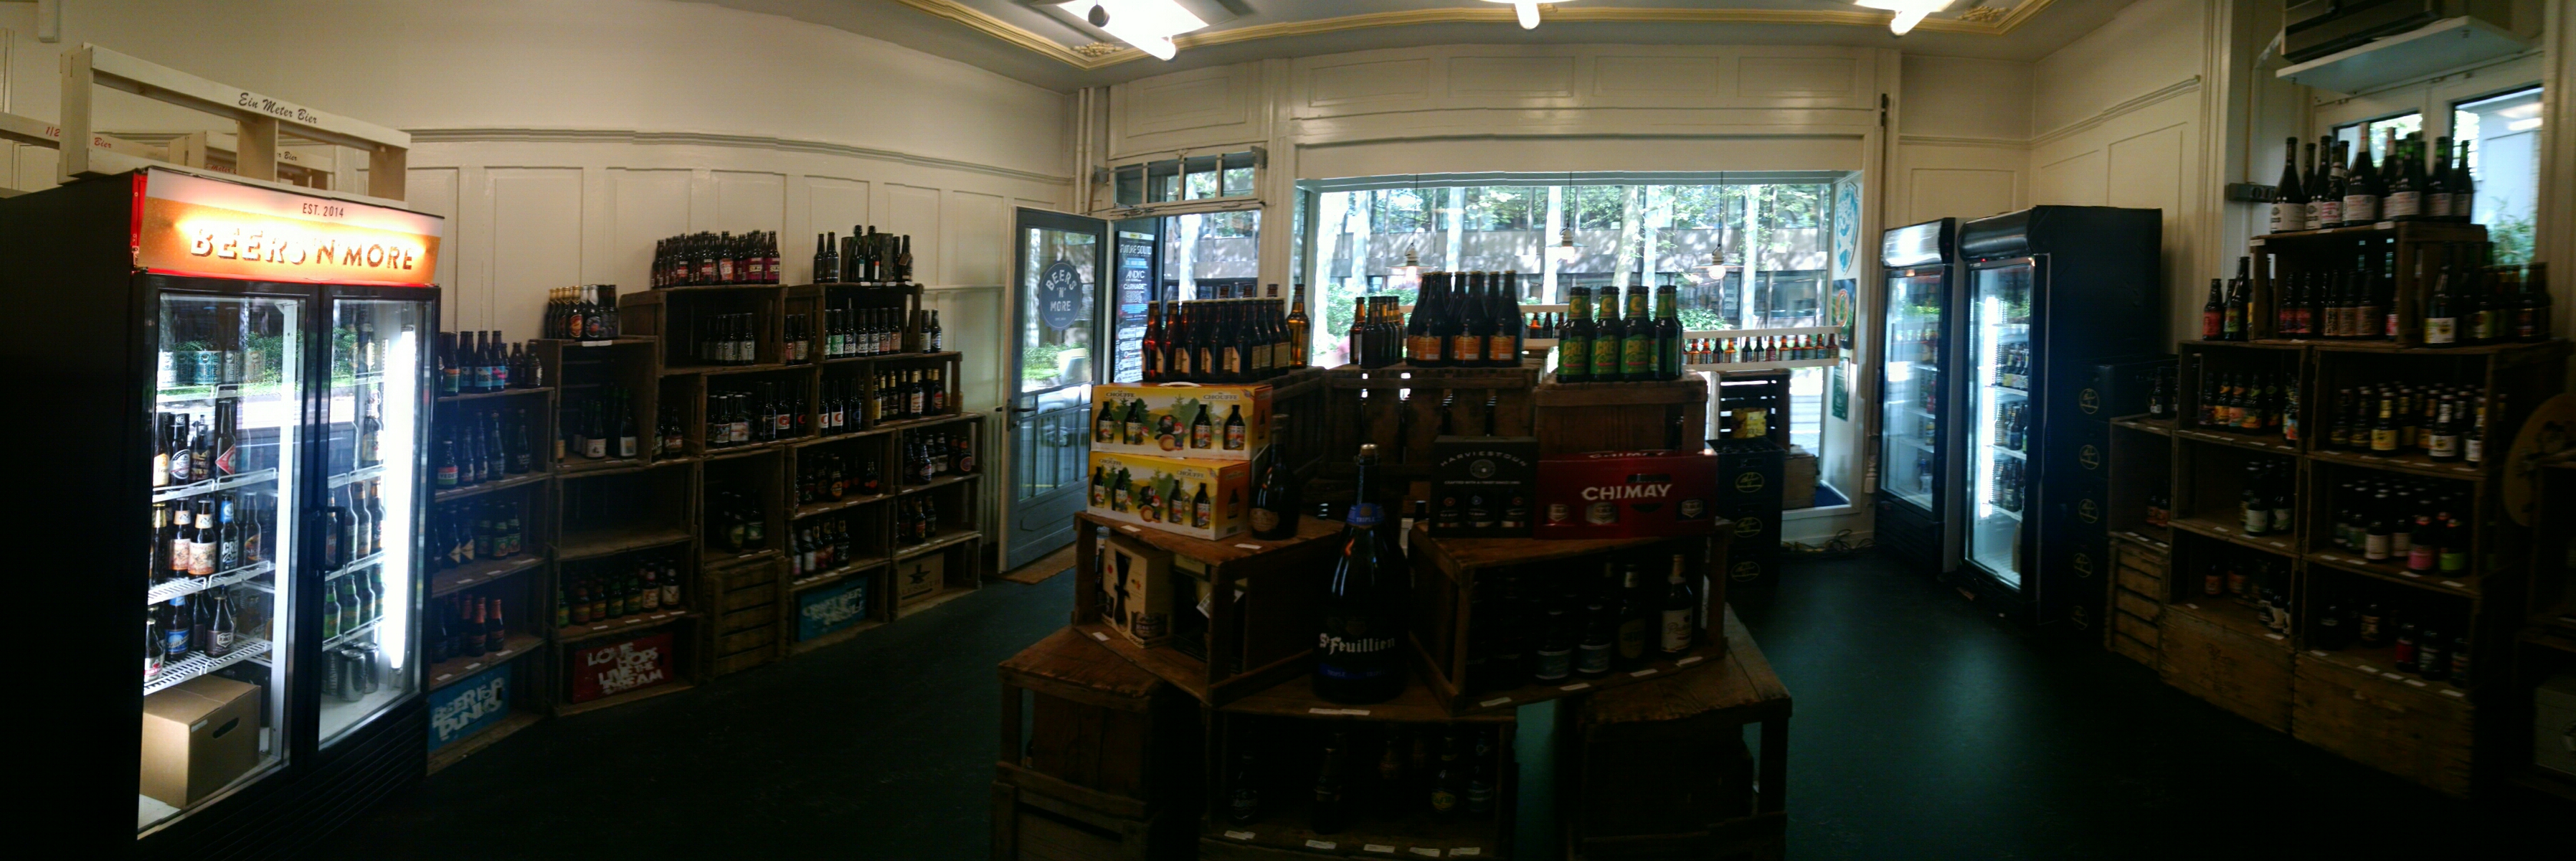
\includegraphics[width=0.9\linewidth]{figures/BeersNMore_panorama.jpg}
\end{center}
\caption{Panorama of BeersNMore interior, displaying a high number of features}
\label{fig:panorama}
\end{figure*}
OpenNI and OpenCV are used to acquire RGB images and depth maps from a Kinect.
The two output images are stored with the same timestamps. The code used for
this step is provided by our supervisor, Bernhard Zeisl.

It is worth noting that the Kinect returns depth in mm in range $[0, 10000]$
which is stored as a 16-bit unsigned integer. Camera parameters are taken from
\cite{smisek20133d} and used in methods in the following steps.

While acquiring data, we attempt to find areas with sufficient potential
features and try to maximise the overlap between each shot to retain enough
correspondences.

This resulted in the BeersNMore dataset, taken at a craft beer shop on
Universit\"atstrasse. The interior of the shop (as seen in figure \ref{fig:panorama}) exhibits
numerous unique and repeating features in the form of labelled beer bottles
boxes, and crates. The dataset consists of 229 RGB and depth images.



%-------------------------------------------------------------------------

\subsection{Feature detection and matching}\label{sec:extractfeature}

For each given RGB image, SIFT features are found, and 128-dimensional are
descriptors calculated. Standard OpenCV parameters are used for this step.
In each image, around 1000 to 2000 features are found.

A matching algorithm is then run between all potential image pairs. This is
an $\mathcal{O}(n^2)$ operation. The matcher computes the euclidian distances of the $i$-th descriptor in one image to all descriptors in the other image and returns the descriptor with minimum distance as the match to descriptor $i$. This produces numerous
incorrect matches, often visible by the violation of epipolar geometry.

The matching is therefore performed in a bi-directional manner, both from image
$i$ to $j$, and $j$ to $i$, so that only consistent matches are kept. This results in a better sample of matches. RANSAC
can be used in the camera registration step to further eliminate outliers.



%-------------------------------------------------------------------------

\subsection{Pairwise camera pose estimation}

The previous step yields a list of image pairs which have matching features.
As in equation \ref{eqn:backprojection}, given the camera matrix $K$, the discovered features $m_{i} = (u,v)^{T}$ from image $i$ can be projected into 3D space
using its depth map values $\rho$. These 3D points are then reprojected into image $j$ (see figure \ref{fig:reg}). The 3D points $P_{i}$ and their corresponding 2D matches $m^i_{j}$ in image $j$ are fed into OpenCV's EPnP solver, which computes the camera pose $i$ w.r.t camera $j$, $T_{ji} = \left(R_{ji}, t_{ji}\right)$ by minimising reprojection error $e$, as defined in equation \ref{eqn:reprojerror} in a RANSAC manner.

\begin{align}
P &= \rho K^{-1} \begin{pmatrix}
u\\v\\1
\end{pmatrix} \label{eqn:backprojection}\\
e &= \sqrt{\norm{\pi\left(P_{i};R_{ji},t_{ji}\right)-m^i_{j}}^2},\label{eqn:reprojerror}
\end{align}
where $\pi$ denotes the projection function \[
\rho
\begin{pmatrix}
\pi\left(P;R,t\right)\\1
\end{pmatrix} = KR\left(P+t\right).
\]


\begin{figure}[t]
\begin{center}
   \includegraphics[width=0.9\linewidth]{figures/registration.pdf}
\end{center}
\caption{Pairwise camera pose registration. Features of camera $i$ are unprojected into 3D space and the reprojection errors (red) are minimised.}
\label{fig:reg}
\end{figure}

The mentioned solver also identifies outlier matches via RANSAC. Only inliers
are retained to improve any further optimisations. To ensure that only good
image pairs are retained, we also filter these image pairs based on an absolute
minimum number of inliers of 30. If two images have less then 30 feature matches
which are inliers in the registration process, it is assumed that the image pair
is not good enough for subsequent steps.

Similar to the feature matching step, the PnP solver is run in both directions,
projecting 3D points from image $i$ into image $j$, and projecting 3D points
from image $j$ into image $i$. This allows for two things, (1) validation of registration result and (2) the averaging of
pose estimates to improve accuracy. In particular, the registration of a camera pair (i,j) is considered successful, only when the rotational vector $r_{ij}$ and $r_{ji}$ from the bi-directional registration are anti-parallel (equation \ref{eqn:check1}) and have similar magnitude (equation \ref{eqn:check2}).

\begin{align}
\norm{\frac{r_{ij}}{\norm{r_{ij}}} + \frac{r_{ji}}{\norm{r_{ji}}}} < 0.2
\label{eqn:check1}\\
\abs{\norm{r_{ij}} - \norm{r_{ji}}} < 0.2\label{eqn:check2}
\end{align}
The final output from this step is a list of camera pairs which are deemed to
have good matching features, and associated pairwise camera pose estimates.


%-------------------------------------------------------------------------

\subsection{Transform to global coordinate system}

The final goal of this SfM pipeline is to combine the data from all images
acquired. To do so, previously acquired pairwise camera pose estimates must
be transformed into a single coordinate frame.

\begin{figure}[t]
\begin{center}
   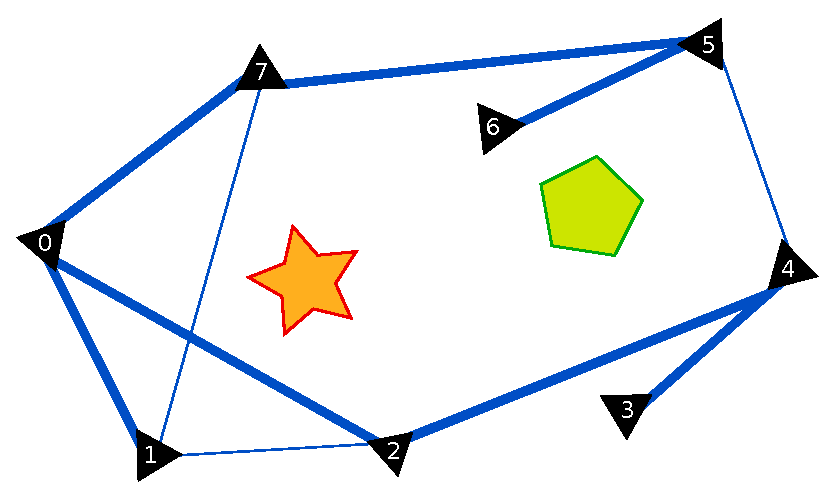
\includegraphics[width=0.9\linewidth]{figures/spanning_tree.eps}
\end{center}
\caption{An example of a minimum spanning tree in terms of this pipeline}
\label{fig:spanning}
\end{figure}

The 0th camera is selected to be the reference coordinate frame. A breadth-first
algorithm is used to construct a minimum spanning tree with cameras as nodes and
the existence of camera pose estimate as edges (whether an image pair exists).

An example of such a spanning tree structure can be seen in figure
\ref{fig:spanning}. 
The spanning tree can be walked to calculate camera pose estimates relative to
the 0th camera as in equation \ref{eqn:globalpose}. Having the global poses, one can obtain the 3D keypoints in global frame using equation \ref{eqn:globalpoint}, where $P^{i}_{k}$ denotes the $i$-th keypoints in $k$-th camera and $P^{i}_{g,k}$ denotes this point transformed in global frame.

\begin{align}\label{eqn:globalpose}
R_{k} &= R_{kj}R_{ji}\ldots R_{0}\nonumber\\
t_{k} &= t_{kj}+t_{ji}+\ldots t_{0}\\
P^{i}_{g,k} &= R_{k}^T P^{i}_{k} - t_{k} \label{eqn:globalpoint}
\end{align}

\begin{figure}[t]
\begin{center}
   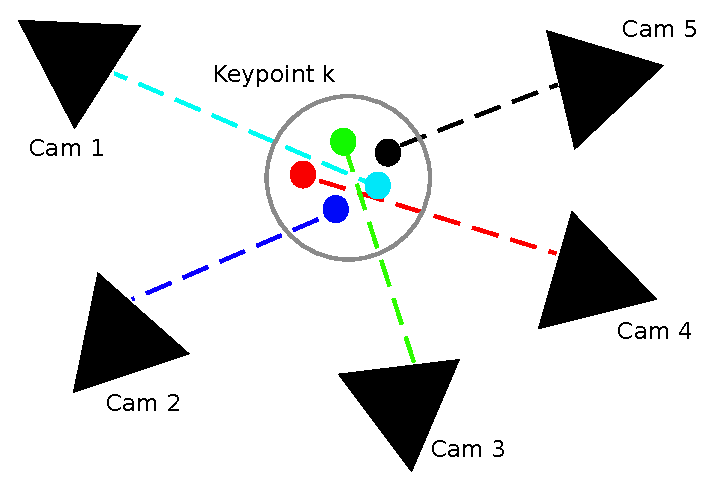
\includegraphics[width=0.9\linewidth]{figures/clusters.eps}
\end{center}
\caption{An example of a cluster of keypoint pose estimations}
\label{fig:clusters}
\end{figure}

The outcome of this step needs to be a cloud of keypoints and camera pose
estimates in global coordinate frame. However, each keypoint is observed by a
minimum of two cameras, resulting in a cluster of keypoint coordinate estimates.
This is illustrated in figure \ref{fig:clusters}.
The centre of mass (CoM) of this cluster is calculated by averaging the
coordinate estimations as in equation \ref{eqn:CoM} \cite{reckerdepth}. This results in a single keypoint coordinate estimate,
and consequently an initial point cloud of sparse features.
\begin{equation}\label{eqn:CoM}
P^{i}_{g} = \sum_{k}{P^{i}_{g,k}}
\end{equation}

%-------------------------------------------------------------------------

\subsection{Bundle adjustment}
With global keypoint and camera pose estimates, it is now possible to perform a global optimisation known as bundle adjustment. This step takes consideration of all estimated 3D points and camera pose into consideration and minimizes a predefined cost function, that reflects the reconstruction quality. Conventionally, this the total reprojection error (as in equation \ref{eqn:baNoD} is used as cost function.

\begin{equation}\label{eqn:baNoD}
\sum_{R_k,t_k}\sum_{P_i}{\norm{\pi\left(P_i;R_k,t_k\right)-m^i_{k}}}^2,
\end{equation}

To this end, having extra depth values of all 3D points, we altered the cost function to exploit this information in hope of an improvement in the reconstruction quality. As can in figure \ref{fig:baCost} and equation \ref{eqn:baD} ,relative error in depth value is incorporated as an extra term, where $d^i_k$ and $\rho^i_k$ denote the measured and estimated depth value respectively.

\begin{equation}\label{eqn:baD}
\sum_{R_k,t_k}\sum_{P_i}{\norm{\pi\left(P_i;R_k,t_k\right)-m^i_{k}}^2+\left\lvert\dfrac{d^i_k-\rho^i_k}{d^i_k}\right\rvert ^2}
\end{equation}

To improve the robustness of this optimization, cauchy loss function $\rho(s) = \log(1+s)$ is utilised which decrease the weight of outliers in the cost function, so that they do not overly influence the final solution.

The result and comparison of both cost functions is shown in section \ref{sec:result}.

\begin{figure}[t]
\begin{center}
   \includegraphics[width=0.9\linewidth]{figures/ba.pdf}
\end{center}
\caption{TODO: BA caption}
\label{fig:baCost}
\end{figure}


%-------------------------------------------------------------------------

\section{Results and discussion}\label{sec:result}

\begin{figure*}
\centering

   \begin{subfigure}[b]{1.0\columnwidth}
   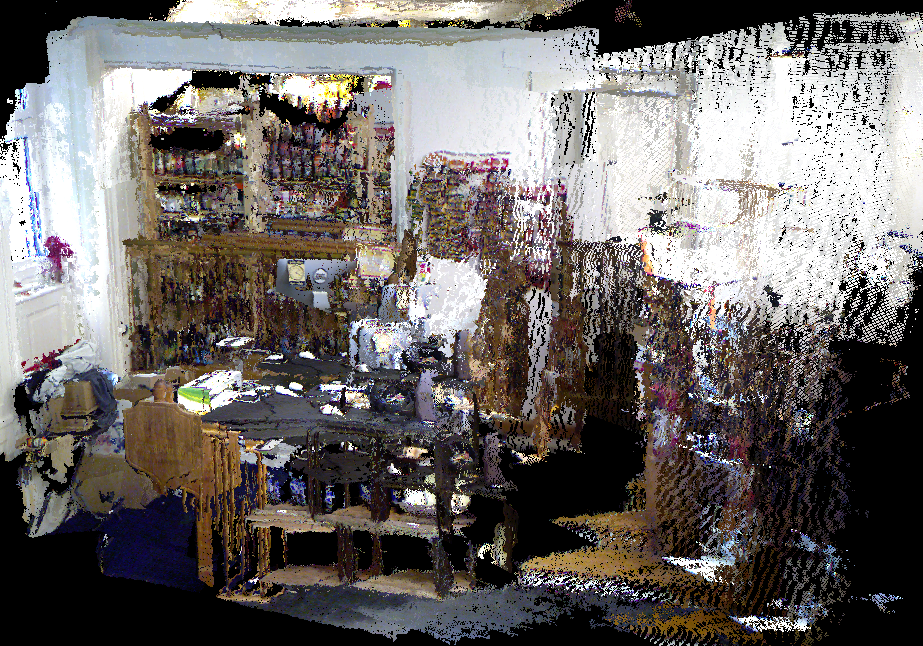
\includegraphics[width=\textwidth]{figures/result_small_noBA.png}
   \caption{Before BA}
   \label{fig:beforeBA}
   \end{subfigure}
   \hfill
   \begin{subfigure}[b]{1.0\columnwidth}
   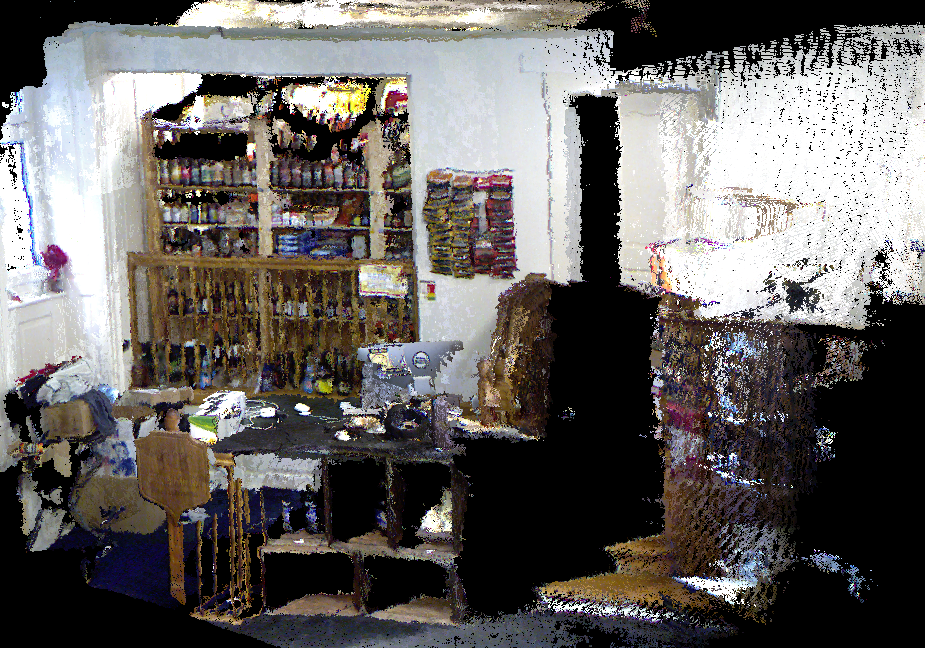
\includegraphics[width=\textwidth]{figures/result_small_BA_noD.png}
   \caption{After BA}
   \label{fig:afterBA}
   \end{subfigure}

\caption{3D reconstruction using a 37-image subset of data. An improvement in
reconstruction quality can be seen after the bundle adjustment step.}
\label{fig:3Dsmall}
\end{figure*}

The pipeline works very well on small datasets which cover an area well with
numerous overlapping shots. The resulting dense reconstruction is of high
quality and alignment is noticably improved with bundle adjustment. This can be
seen in figures \ref{fig:beforeBA} and \ref{fig:afterBA} where a rough initial
estimate is refined through bundle adjustment.

\begin{figure*}
\centering

   \begin{subfigure}[b]{1.0\columnwidth}
   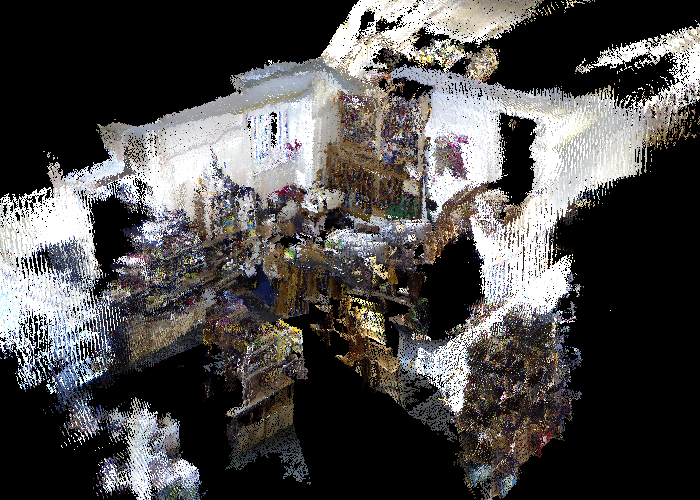
\includegraphics[width=\textwidth]{figures/result_large_BA_noD.png}
   \caption{BA without depth}
   \label{fig:BA_noD}
   \end{subfigure}
   \hfill
   \begin{subfigure}[b]{1.0\columnwidth}
   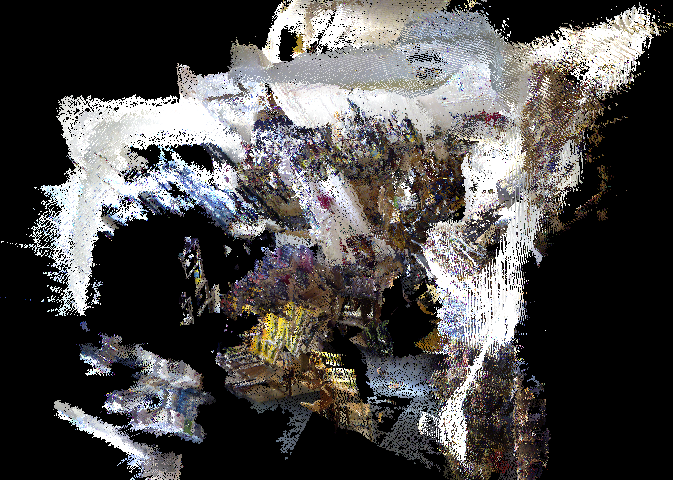
\includegraphics[width=\textwidth]{figures/result_large_BA_D.png}
   \caption{BA with depth}
   \label{fig:BA_withD}
   \end{subfigure}

\caption{3D reconstruction using the full dataset (226 images). With the depth
term added to the bundle adjustment step, the reconstruction is no longer
successful. It can also be seen the the reconstruction quality drops for the
larger dataset.}
\label{fig:3Dlarge}
\end{figure*}

However, it performs less well when some correspondences are weak and thus
prevents the final spanning tree from spanning all cameras. This results in a
partial reconstruction of the scene. This is also evident when there are
sufficient correspondences for the spanning tree construction to propagate,
but not enough for a good estimate of camera pose to be made. This results in a
lower quality reconstruction (figure \ref{fig:3Dlarge}).

The lack of correspondences is not only due to issues in data acquisition, but
also due to varying lighting conditions. For example, the light bleeding from
the beer fridges and windows caused feature matches to succeed less well.

We attempt to use depth data in our bundle adjustment step. This was in hopes of
improving the final reconstruction accuracy. It can be seen however in figures
\ref{fig:BA_noD} and \ref{fig:BA_withD} that using depth data can sometimes
prevent the bundle adjustment step from executing successfully. This could be
due to the limited resolution of depth data compared to reprojection errors.

\begin{figure}
\begin{center}
   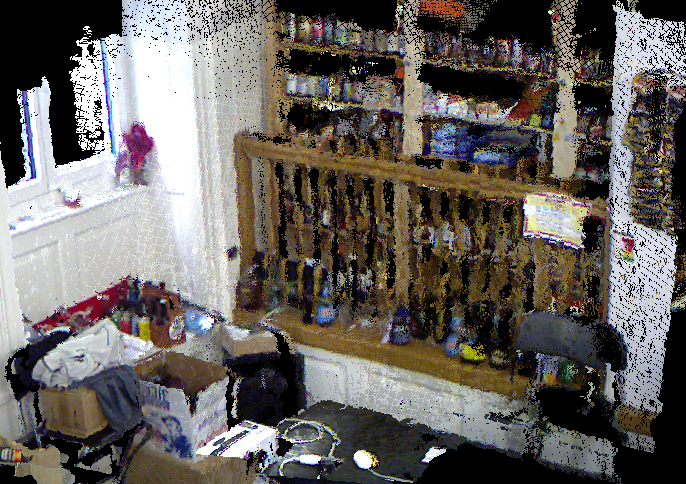
\includegraphics[width=0.9\linewidth]{figures/result_tiny_noBA.png}
\end{center}
\caption{3D reconstruction result using just 6 images}
\label{fig:3D_6images}
\end{figure}

Nonetheless, the pipeline works well in general, and does not require specific
parameters and is thus general purpose. Even with as few as 6 images, an
accurate dense reconstruction is possible (figure \ref{fig:3D_6images}) and this can be extended to larger
areas with more images with sufficient correspondences.


%-------------------------------------------------------------------------

\section{Conclusion}

A Structure from Motion pipeline taking advantage of both RGB and depth
information was successfully implemented. This involved all steps starting
from the acquisition of data to the visualisation of the final 3D model. A
good understanding of all parts of the pipeline as well as associated technology
was required.

One of the goals of this project was to investigate the improvements which can
be made by incorporating the depth information provided by the Kinect. We can
show that the camera registration step works quite well with depth data, as can
be seen in the final reconstructions. It cannot be said however that depth data
can improve the bundle adjustment step. Our initial assessment shows that the
low resolution of depth data ($2^{11}$ bits) can result in a degradation in
quality of the final model, but this may require more analysis.

It can be claimed that incorporating depth data into the pipeline makes it more
robust. This is because depth data is used in multiple steps such as camera
registration and the finding of centre-of-mass of keypoint pose clusters instead
of periodic bundle adjustment. A final bundle adjustment is enough to produce a
high quality final model.

One assessment which may be helpful is the comparison of our 2D-3D registration
method against a more conventional 2D-2D registration as well as 3D-3D
registration using depth data from both images in a pair. This would further
inform us whether depth data is helpful in structure from motion and in which
steps. We propose this as future work in this area.


%-------------------------------------------------------------------------

\section*{Work distribution}

The authors worked together weekly and thus shared workload fairly.

Park focused more infrastructure, spanning tree, and visualisation, while Wang
focused more on camera registration, clusters finding and bundle adjustment.

Data acquisition was done with cooperation from Jonathan, the owner of craft
beer shop, BeersNMore.

We thank Pavol Vyhlidal, An-phi Nguyen, and Federico Danieli for their support
and enthusiasm.


%-------------------------------------------------------------------------

{\small
\bibliographystyle{ieeetr}
\bibliography{egbib}
}

\end{document}
